% Cole Nielsen niels538@umn.edu
% EE 2002 Spring 2015
% Formal Lab Report 1

%----------------------------------------------------------------------------------------
%	PACKAGES AND DOCUMENT CONFIGURATIONS
%----------------------------------------------------------------------------------------

\documentclass[12pt]{article}

\usepackage{circuitikz}
\usepackage{graphicx}
\usepackage{subcaption}
\usepackage[top=1in, bottom= 1in, left=1in, right= 1in]{geometry}
\setlength\parindent{0pt}
\usepackage{fancyhdr}
\pagestyle{fancy}
\usepackage{textcomp}
\usepackage{tikz}
\usepackage{siunitx}
\usepackage{placeins}
\usepackage{titlesec}
\usepackage{cancel} 
\usepackage{tikz}
\usetikzlibrary{shapes.geometric, arrows}
\tikzstyle{box} = [rectangle, rounded corners, minimum width = 3cm, minimum height = 1cm, text centered, draw = black]
\tikzstyle{arrow} = [thick,->,>=stealth]
\usepackage{placeins}

\usepackage{listings}
\usepackage{color}

\definecolor{dkgreen}{rgb}{0,0.6,0}
\definecolor{gray}{rgb}{0.5,0.5,0.5}
\definecolor{mauve}{rgb}{0.58,0,0.82}

\lstset{frame=tb,
  language=,
  aboveskip=3mm,
  belowskip=3mm,
  showstringspaces=false,
  columns=flexible,
  basicstyle={\small\ttfamily},
  numbers=none,
  numberstyle=\tiny\color{gray},
  keywordstyle=\color{blue},
  commentstyle=\color{dkgreen},
  stringstyle=\color{mauve},
  breaklines=true,
  breakatwhitespace=true,
  tabsize=3
}

%----------------------------------------------------------------------------------------
%	DOCUMENT INFORMATION
%----------------------------------------------------------------------------------------

\title{Lab 1 Report\\ \vspace{0.3 in} EE 4111}

\newcommand{\mymeter}[2]{   	% #1 = name , #2 = rotation angle
 \begin{scope}[transform shape,rotate=#2]
   \draw[thick] (#1)node(){$\mathbf V$} circle (11pt);
   \draw[rotate=45,-latex] (#1)  +(-17pt,0) --+(17pt,0);
 \end{scope}
}
\author{Cole \textsc{Nielsen}}
\date{Spring 2016}
\begin{document}
\maketitle 
\pagebreak
%---------------------------------------------------------------------------------------
%----------------------------------------------------------------------------------------
%	Introduction
%----------------------------------------------------------------------------------------
\section*{Task 2}
The objective of this task was to make a family of I-V characteritic curves for the given MOSFET model. Below is the circuit used with labeled nodes. Underneath the circuit schematic is the netlist for this circuit (body effect is ignored for this part). The family of I-V curves were generated by sweeping the drain-to-source voltage (Vds) for five different gate to source voltages (Vgs), done with the .DC directive. The output was plotted in Cosmoscope.
\FloatBarrier
\begin{figure}[h!]
\begin{center}
 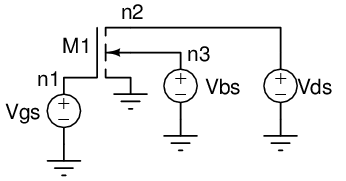
\includegraphics[scale=0.7]{./2.png}
\end{center}
\end{figure}
\FloatBarrier
\begin{lstlisting}
mosfet i-v curve
.OPTIONS LIST NODE POST
.DC Vds 0V 10V 100mV	Vgs 0 8V 2V
.PRINT DC V(3) I1(M1)

Vgs 1 0 DC 3
Vds 2 0 DC 1
M1 2 1 0 0 CMOSN W = 10U L = 1.5U

.MODEL CMOSN NMOS ( LEVEL = 3 
+ TOX = 1.4E-8  NSUB   = 1E17 GAMMA  = 0.5483559          
+ PHI = 0.7 VTO = 0.7640855 DELTA = 3.0541177 
+ UO = 662.6984452 ETA = 3.162045E-6 THETA  = 0.1013999          
+ KP  = 1.259355E-4 VMAX   = 1.442228E5 KAPPA  = 0.3             
+ RSH = 7.513418E-3  NFS = 1E12      TPG    = 1                     
+ XJ     = 3E-7  LD  = 1E-13  WD = 2.334779E-7
+ CGD = 2.15E-10 CGSO   = 2.15E-10   CGBO   = 1E-10        
+ C = 4.258447E-4 PB  = 0.914037   MJ     = 0.435903 
+ CJSW   = 3.147465E-10    MJSW   = 0.1977689       )                                     

.END
\end{lstlisting}
In the following plot notice the parabolic ($\propto V_{ov}^2$) growth of I$_d$, as well as the Early effect causing the saturation region to have a slope.
\FloatBarrier
\begin{figure}[h!]
\begin{center}
 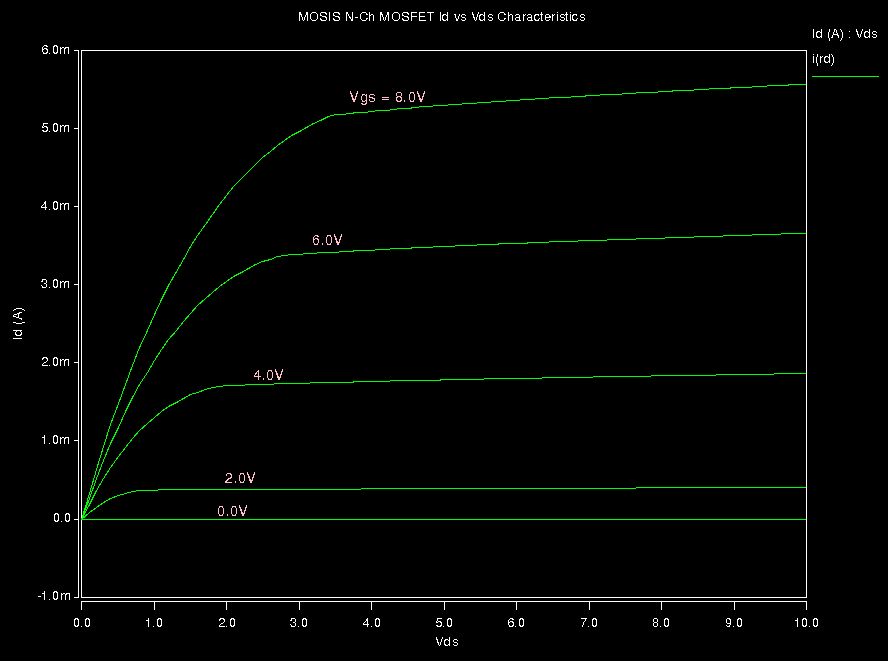
\includegraphics[scale=0.35]{./mftiv.png}
\end{center}
\end{figure}
\FloatBarrier
The second part of this task was to investigate how the body effect (gamma parameter) affects the I-V characteristic of a MOSFET. This was done by modififying the netlist to include a body to source voltage (Vbs) and then keeping Vds constant while sweeping Vbs. The body to source voltage is always kept at a negative potential to ground, as reversing the polarity would forward bias the source body junction.
\begin{lstlisting}
mosfet i-v curve
.OPTIONS LIST NODE POST
.DC Vgs 0V 2.5V 5mV	Vbs 0 -3V 1V
.PRINT DC V(1) I1(M1)

Vgs 1 0 DC 3V
Vds 2 0 DC 0.1V
Vbs 3 0 DC 1V
M1 2 1 0 3 CMOSN W = 10U L = 1.5U

.MODEL CMOSN NMOS ( LEVEL = 3 
+ TOX = 1.4E-8  NSUB   = 1E17 GAMMA  = 0.5483559          
+ PHI = 0.7 VTO = 0.7640855 DELTA = 3.0541177 
+ UO = 662.6984452 ETA = 3.162045E-6 THETA  = 0.1013999          
+ KP  = 1.259355E-4 VMAX   = 1.442228E5 KAPPA  = 0.3             
+ RSH = 7.513418E-3  NFS = 1E12      TPG    = 1                     
+ XJ     = 3E-7  LD  = 1E-13  WD = 2.334779E-7
+ CGD = 2.15E-10 CGSO   = 2.15E-10   CGBO   = 1E-10        
+ C = 4.258447E-4 PB  = 0.914037   MJ     = 0.435903 
+ CJSW   = 3.147465E-10    MJSW   = 0.1977689       )                                     

.END
\end{lstlisting}
It should be noted that the body effect (gamma) affects the Id-Vgs characteristic by increasing the Vgs needed for a current with a greater Vbs. This is an important parameter to understand and to design for when designing microelectronics as it has a large impact on circuit behavior.
\FloatBarrier
\begin{figure}[h!]
\begin{center}
 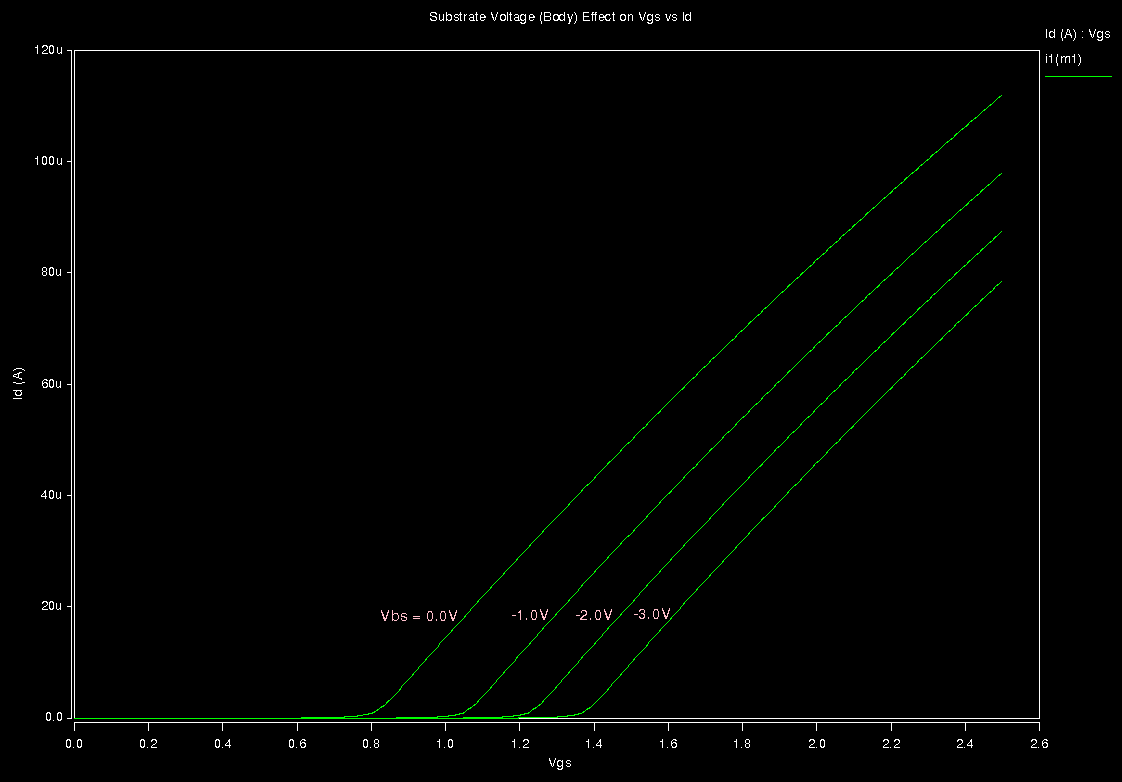
\includegraphics[scale=0.35]{./body.png}
\end{center}
\end{figure}
\FloatBarrier

\section*{Task 3}
The objective of this task was to create a netlist for the active cascode circuit of figure 3.41 in Grey and Meyer. The circuit is designed have Vbias and Vi set such that the drain current is approximately 500$\mu$A. The bodies of both transistors are connected to ground, and the OP AMP feedback amplifier is modeled by an ideal amplifier. The current was set to 500$\mu$A by approximately calculating the $V_{ov}$ using $V_{ov} = \frac{1}{2}\textnormal{KP}\times V_{ov}^2$, and then setting Vbias to that voltage. Vi was set to Vto plus Vov. This was then simulated using an DC operating point simulation. The values of Vbias and Vi were then tweaked for the drain current to be closer to 500$\mu$A. As follows is the circuit diagram and netlist.
\FloatBarrier 
\begin{figure}[h!]
\begin{center}
 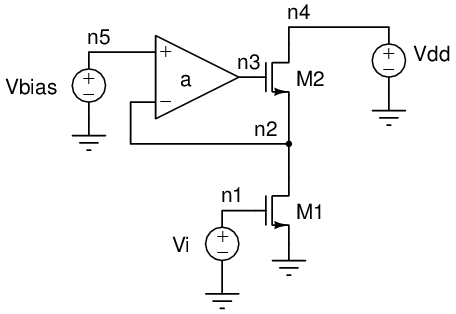
\includegraphics[scale=0.7]{./3.png}
\end{center}
\end{figure}
\FloatBarrier
\begin{lstlisting}
active cascode
.OPTIONS LIST NODE POST
.OP
.PRINT DC V(n1) V(n4) I1(M2)  

Vdd n4 0 DC 8V 
Vbias n5 0 DC 1.6V
Vi n1 0 DC 2.25V 
M1 n2 n1 0 0 CMOSN W = 10U L = 1.5U
M2 n4 n3 n2 0 CMOSN W = 10U L = 1.5U
Eopamp n3 0 OPAMP n5 n2 

.MODEL CMOSN NMOS ( LEVEL = 3 
+ TOX = 1.4E-8  NSUB   = 1E17 GAMMA  = 0.5483559          
+ PHI = 0.7 VTO = 0.7640855 DELTA = 3.0541177 
+ UO = 662.6984452 ETA = 3.162045E-6 THETA  = 0.1013999          
+ KP  = 1.259355E-4 VMAX   = 1.442228E5 KAPPA  = 0.3             
+ RSH = 7.513418E-3  NFS = 1E12      TPG    = 1                     
+ XJ     = 3E-7  LD  = 1E-13  WD = 2.334779E-7
+ CGD = 2.15E-10 CGSO   = 2.15E-10   CGBO   = 1E-10        
+ C = 4.258447E-4 PB  = 0.914037   MJ     = 0.435903 
+ CJSW   = 3.147465E-10    MJSW   = 0.1977689       )                                     

.END
\end{lstlisting}
Below is the data from the output listing file of the DC operaing point of the two MOSFETS. The drain currents are both close to 500 $\mu$A and both devices are in saturation.
\begin{lstlisting}
 subckt                        
 element  0:m1       0:m2      
 model    0:cmosn    0:cmosn   
 region     Saturati   Saturati
  id       508.1523u  503.0331u
  ibs        0.       -16.0000f
  ibd      -16.0000f  -80.0000f
  vgs        2.2500     2.5078 
  vds        1.6000     6.4000 
  vbs        0.        -1.6000 
  vth      750.7243m    1.1050 
  vdsat      1.0655     1.0611 
  vod        1.4993     1.4028 
  beta     541.3695u  545.4733u
  gam eff  514.7031m  495.2495m
  gm       561.4416u  601.1679u
  gds        7.6704u    4.2889u
  gmb        0.        95.8735u
  cdtot      2.2252f    2.4510f
  cgtot     28.1535f   28.3405f
  cstot     25.6637f   25.6637f
  cbtot    264.6000a  225.9071a
  cgs       25.6637f   25.6637f
  cgd        2.2252f    2.4510f
\end{lstlisting}
\section*{Task 4}
Task 4 uses the same netlist as Task 3, however modified to have an adjustable gain. The objective of this part is to find the output resistance looking into the drain of M2. Since this is a cascode configuration, the output inpedence should be extremely high, especially if the drain to source voltage of M1 is held constant across M1 due to the feedback amplifier and Vi is held constant. Holding these voltages constant effectively negate the Early effect for M1, which essentially elimates the $r_o$ term for that transistor in the small signal domain. It is expected that the high gain the opamp has, the better the Vds of M2 will stay constant, and the higher the output resistance will be. The output resistance was found by adding a AC voltage to the the supply voltage connected to the drain of M2. Running an AC simulation at a low frequency (to avoid capacitive effects) allows us to see the small signal current that flows into the active cascode, and the output resistance can therefore be calculated as the ration of the AC voltage to the AC current. Below is the netlist for this circuit.
\begin{lstlisting}
active cascode
.OPTIONS LIST NODE POST 
.PRINT AC V(n4) I1(M2) PAR('V(n4)/I1(M2)')
.AC DEC 1 10 100

Vdd n4 0 DC 8V AC 1 SIN (0 1 100)
Vbias n5 0 DC 1.6V
Vi n1 0 DC 2.25V 
M1 n2 n1 0 0 CMOSN W = 10U L = 1.5U
M2 n4 n3 n2 0 CMOSN W = 10U L = 1.5U
E0 n3 0 n5 n2 1000

.MODEL CMOSN NMOS ( LEVEL = 3 
+ TOX = 1.4E-8  NSUB   = 1E17 GAMMA  = 0.5483559          
+ PHI = 0.7 VTO = 0.7640855 DELTA = 3.0541177 
+ UO = 662.6984452 ETA = 3.162045E-6 THETA  = 0.1013999          
+ KP  = 1.259355E-4 VMAX   = 1.442228E5 KAPPA  = 0.3             
+ RSH = 7.513418E-3  NFS = 1E12      TPG    = 1                     
+ XJ     = 3E-7  LD  = 1E-13  WD = 2.334779E-7
+ CGD = 2.15E-10 CGSO   = 2.15E-10   CGBO   = 1E-10        
+ C = 4.258447E-4 PB  = 0.914037   MJ     = 0.435903 
+ CJSW   = 3.147465E-10    MJSW   = 0.1977689       )                                     
*

.END
\end{lstlisting}
This circuit was simulated for feedback gain settings of 1, 10, 100 and 1000. Below are the results plotted in logscale. The impedence was extremely high as expected, topping off at 18 G$\Omega$ for \textit{a} = 1000. As expected, output resistance grows with gain, almost exponentially. It should be noted that the active cascode was unable to mantain a drain current of 100$\mu$A  with a gain setting of 1. \\
\begin {figure}[htb!]
  \begin{center}
    	\resizebox{0.6\textwidth}{!}{% GNUPLOT: LaTeX picture
\setlength{\unitlength}{0.240900pt}
\ifx\plotpoint\undefined\newsavebox{\plotpoint}\fi
\begin{picture}(1500,900)(0,0)
\sbox{\plotpoint}{\rule[-0.200pt]{0.400pt}{0.400pt}}%
\put(231.0,131.0){\rule[-0.200pt]{4.818pt}{0.400pt}}
\put(211,131){\makebox(0,0)[r]{ 1}}
\put(1419.0,131.0){\rule[-0.200pt]{4.818pt}{0.400pt}}
\put(231.0,170.0){\rule[-0.200pt]{2.409pt}{0.400pt}}
\put(1429.0,170.0){\rule[-0.200pt]{2.409pt}{0.400pt}}
\put(231.0,221.0){\rule[-0.200pt]{2.409pt}{0.400pt}}
\put(1429.0,221.0){\rule[-0.200pt]{2.409pt}{0.400pt}}
\put(231.0,247.0){\rule[-0.200pt]{2.409pt}{0.400pt}}
\put(1429.0,247.0){\rule[-0.200pt]{2.409pt}{0.400pt}}
\put(231.0,260.0){\rule[-0.200pt]{4.818pt}{0.400pt}}
\put(211,260){\makebox(0,0)[r]{ 10}}
\put(1419.0,260.0){\rule[-0.200pt]{4.818pt}{0.400pt}}
\put(231.0,299.0){\rule[-0.200pt]{2.409pt}{0.400pt}}
\put(1429.0,299.0){\rule[-0.200pt]{2.409pt}{0.400pt}}
\put(231.0,350.0){\rule[-0.200pt]{2.409pt}{0.400pt}}
\put(1429.0,350.0){\rule[-0.200pt]{2.409pt}{0.400pt}}
\put(231.0,376.0){\rule[-0.200pt]{2.409pt}{0.400pt}}
\put(1429.0,376.0){\rule[-0.200pt]{2.409pt}{0.400pt}}
\put(231.0,389.0){\rule[-0.200pt]{4.818pt}{0.400pt}}
\put(211,389){\makebox(0,0)[r]{ 100}}
\put(1419.0,389.0){\rule[-0.200pt]{4.818pt}{0.400pt}}
\put(231.0,428.0){\rule[-0.200pt]{2.409pt}{0.400pt}}
\put(1429.0,428.0){\rule[-0.200pt]{2.409pt}{0.400pt}}
\put(231.0,479.0){\rule[-0.200pt]{2.409pt}{0.400pt}}
\put(1429.0,479.0){\rule[-0.200pt]{2.409pt}{0.400pt}}
\put(231.0,505.0){\rule[-0.200pt]{2.409pt}{0.400pt}}
\put(1429.0,505.0){\rule[-0.200pt]{2.409pt}{0.400pt}}
\put(231.0,518.0){\rule[-0.200pt]{4.818pt}{0.400pt}}
\put(211,518){\makebox(0,0)[r]{ 1000}}
\put(1419.0,518.0){\rule[-0.200pt]{4.818pt}{0.400pt}}
\put(231.0,557.0){\rule[-0.200pt]{2.409pt}{0.400pt}}
\put(1429.0,557.0){\rule[-0.200pt]{2.409pt}{0.400pt}}
\put(231.0,608.0){\rule[-0.200pt]{2.409pt}{0.400pt}}
\put(1429.0,608.0){\rule[-0.200pt]{2.409pt}{0.400pt}}
\put(231.0,634.0){\rule[-0.200pt]{2.409pt}{0.400pt}}
\put(1429.0,634.0){\rule[-0.200pt]{2.409pt}{0.400pt}}
\put(231.0,647.0){\rule[-0.200pt]{4.818pt}{0.400pt}}
\put(211,647){\makebox(0,0)[r]{ 10000}}
\put(1419.0,647.0){\rule[-0.200pt]{4.818pt}{0.400pt}}
\put(231.0,686.0){\rule[-0.200pt]{2.409pt}{0.400pt}}
\put(1429.0,686.0){\rule[-0.200pt]{2.409pt}{0.400pt}}
\put(231.0,737.0){\rule[-0.200pt]{2.409pt}{0.400pt}}
\put(1429.0,737.0){\rule[-0.200pt]{2.409pt}{0.400pt}}
\put(231.0,763.0){\rule[-0.200pt]{2.409pt}{0.400pt}}
\put(1429.0,763.0){\rule[-0.200pt]{2.409pt}{0.400pt}}
\put(231.0,776.0){\rule[-0.200pt]{4.818pt}{0.400pt}}
\put(211,776){\makebox(0,0)[r]{ 100000}}
\put(1419.0,776.0){\rule[-0.200pt]{4.818pt}{0.400pt}}
\put(231.0,131.0){\rule[-0.200pt]{0.400pt}{4.818pt}}
\put(231,90){\makebox(0,0){ 1}}
\put(231.0,756.0){\rule[-0.200pt]{0.400pt}{4.818pt}}
\put(352.0,131.0){\rule[-0.200pt]{0.400pt}{2.409pt}}
\put(352.0,766.0){\rule[-0.200pt]{0.400pt}{2.409pt}}
\put(423.0,131.0){\rule[-0.200pt]{0.400pt}{2.409pt}}
\put(423.0,766.0){\rule[-0.200pt]{0.400pt}{2.409pt}}
\put(473.0,131.0){\rule[-0.200pt]{0.400pt}{2.409pt}}
\put(473.0,766.0){\rule[-0.200pt]{0.400pt}{2.409pt}}
\put(512.0,131.0){\rule[-0.200pt]{0.400pt}{2.409pt}}
\put(512.0,766.0){\rule[-0.200pt]{0.400pt}{2.409pt}}
\put(544.0,131.0){\rule[-0.200pt]{0.400pt}{2.409pt}}
\put(544.0,766.0){\rule[-0.200pt]{0.400pt}{2.409pt}}
\put(571.0,131.0){\rule[-0.200pt]{0.400pt}{2.409pt}}
\put(571.0,766.0){\rule[-0.200pt]{0.400pt}{2.409pt}}
\put(595.0,131.0){\rule[-0.200pt]{0.400pt}{2.409pt}}
\put(595.0,766.0){\rule[-0.200pt]{0.400pt}{2.409pt}}
\put(615.0,131.0){\rule[-0.200pt]{0.400pt}{2.409pt}}
\put(615.0,766.0){\rule[-0.200pt]{0.400pt}{2.409pt}}
\put(634.0,131.0){\rule[-0.200pt]{0.400pt}{4.818pt}}
\put(634,90){\makebox(0,0){ 10}}
\put(634.0,756.0){\rule[-0.200pt]{0.400pt}{4.818pt}}
\put(755.0,131.0){\rule[-0.200pt]{0.400pt}{2.409pt}}
\put(755.0,766.0){\rule[-0.200pt]{0.400pt}{2.409pt}}
\put(826.0,131.0){\rule[-0.200pt]{0.400pt}{2.409pt}}
\put(826.0,766.0){\rule[-0.200pt]{0.400pt}{2.409pt}}
\put(876.0,131.0){\rule[-0.200pt]{0.400pt}{2.409pt}}
\put(876.0,766.0){\rule[-0.200pt]{0.400pt}{2.409pt}}
\put(915.0,131.0){\rule[-0.200pt]{0.400pt}{2.409pt}}
\put(915.0,766.0){\rule[-0.200pt]{0.400pt}{2.409pt}}
\put(947.0,131.0){\rule[-0.200pt]{0.400pt}{2.409pt}}
\put(947.0,766.0){\rule[-0.200pt]{0.400pt}{2.409pt}}
\put(974.0,131.0){\rule[-0.200pt]{0.400pt}{2.409pt}}
\put(974.0,766.0){\rule[-0.200pt]{0.400pt}{2.409pt}}
\put(997.0,131.0){\rule[-0.200pt]{0.400pt}{2.409pt}}
\put(997.0,766.0){\rule[-0.200pt]{0.400pt}{2.409pt}}
\put(1018.0,131.0){\rule[-0.200pt]{0.400pt}{2.409pt}}
\put(1018.0,766.0){\rule[-0.200pt]{0.400pt}{2.409pt}}
\put(1036.0,131.0){\rule[-0.200pt]{0.400pt}{4.818pt}}
\put(1036,90){\makebox(0,0){ 100}}
\put(1036.0,756.0){\rule[-0.200pt]{0.400pt}{4.818pt}}
\put(1158.0,131.0){\rule[-0.200pt]{0.400pt}{2.409pt}}
\put(1158.0,766.0){\rule[-0.200pt]{0.400pt}{2.409pt}}
\put(1228.0,131.0){\rule[-0.200pt]{0.400pt}{2.409pt}}
\put(1228.0,766.0){\rule[-0.200pt]{0.400pt}{2.409pt}}
\put(1279.0,131.0){\rule[-0.200pt]{0.400pt}{2.409pt}}
\put(1279.0,766.0){\rule[-0.200pt]{0.400pt}{2.409pt}}
\put(1318.0,131.0){\rule[-0.200pt]{0.400pt}{2.409pt}}
\put(1318.0,766.0){\rule[-0.200pt]{0.400pt}{2.409pt}}
\put(1350.0,131.0){\rule[-0.200pt]{0.400pt}{2.409pt}}
\put(1350.0,766.0){\rule[-0.200pt]{0.400pt}{2.409pt}}
\put(1377.0,131.0){\rule[-0.200pt]{0.400pt}{2.409pt}}
\put(1377.0,766.0){\rule[-0.200pt]{0.400pt}{2.409pt}}
\put(1400.0,131.0){\rule[-0.200pt]{0.400pt}{2.409pt}}
\put(1400.0,766.0){\rule[-0.200pt]{0.400pt}{2.409pt}}
\put(1421.0,131.0){\rule[-0.200pt]{0.400pt}{2.409pt}}
\put(1421.0,766.0){\rule[-0.200pt]{0.400pt}{2.409pt}}
\put(1439.0,131.0){\rule[-0.200pt]{0.400pt}{4.818pt}}
\put(1439,90){\makebox(0,0){ 1000}}
\put(1439.0,756.0){\rule[-0.200pt]{0.400pt}{4.818pt}}
\put(231.0,131.0){\rule[-0.200pt]{0.400pt}{155.380pt}}
\put(231.0,131.0){\rule[-0.200pt]{291.007pt}{0.400pt}}
\put(1439.0,131.0){\rule[-0.200pt]{0.400pt}{155.380pt}}
\put(231.0,776.0){\rule[-0.200pt]{291.007pt}{0.400pt}}
\put(30,453){\makebox(0,0){\hspace{-36pt}Ro (M$\Omega$)}}
\put(835,29){\makebox(0,0){Opamp Gain (V/V)}}
\put(835,838){\makebox(0,0){Active Cascode Output Resistance vs Feedback Amplifier Gain}}
\put(231,185){\usebox{\plotpoint}}
\multiput(231.00,185.58)(0.840,0.500){477}{\rule{0.772pt}{0.120pt}}
\multiput(231.00,184.17)(401.398,240.000){2}{\rule{0.386pt}{0.400pt}}
\multiput(634.00,425.58)(1.585,0.499){251}{\rule{1.366pt}{0.120pt}}
\multiput(634.00,424.17)(399.164,127.000){2}{\rule{0.683pt}{0.400pt}}
\multiput(1036.00,552.58)(1.577,0.499){253}{\rule{1.359pt}{0.120pt}}
\multiput(1036.00,551.17)(400.179,128.000){2}{\rule{0.680pt}{0.400pt}}
\put(231.0,131.0){\rule[-0.200pt]{0.400pt}{155.380pt}}
\put(231.0,131.0){\rule[-0.200pt]{291.007pt}{0.400pt}}
\put(1439.0,131.0){\rule[-0.200pt]{0.400pt}{155.380pt}}
\put(231.0,776.0){\rule[-0.200pt]{291.007pt}{0.400pt}}
\end{picture}
}
  \end	{center}
\end {figure}
\FloatBarrier
Below are the numerical values for gain extracted from the simulation output listing files:\\
\begin{center}
\begin{tabular}{l r}
\textit{a = 1} & R$_o$ = 2.6399 M$\Omega$\\
\textit{a = 10} & R$_o$ = 190.01 M$\Omega$\\
\textit{a = 100} & R$_o$ = 1823.2 M$\Omega$\\
\textit{a = 1000} & R$_o$ = 18132 M$\Omega$\\
\end{tabular}
\end{center}
\pagebreak
\section*{Task 5}
The objective of this part was to determine the linear input range of the below source coupled amplifier. The values for Rc and the supply voltages were adjusted to give a subjectively linear region between plus and minus 0.5 volts input differential. Itail was set to 200uA.
\FloatBarrier
\begin{figure}[h!]
\begin{center}
 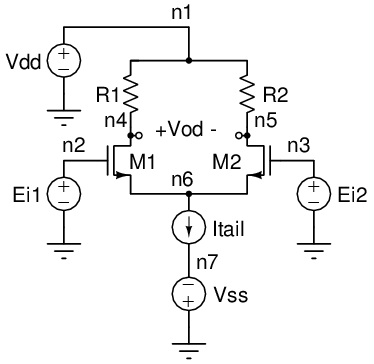
\includegraphics[scale=0.7]{./5.png}
\end{center}
\end{figure}
\FloatBarrier
\begin{lstlisting}
source coupled pair
.OPTIONS LIST NODE POST
.DC Vdiff -0.5 0.5 0.01 $differential voltage sweep
.PRINT DC PAR('V(n3)-V(n2)') PAR('V(n5) - V(n4)') I(Rd1) I(Rd2)

Vdd n1 0 DC 5 
Vss 0 n7 DC 5
Vdiff n10 0 DC 0
Ei1 n2 0 VOL = '-1*V(n10)'	$differential inputs
Ei2 n3 0 VOL = 'V(n10)'		
Rd1 n1 n4 25000
Rd2 n1 n5 25000
M1 n4 n2 n6 n7 CMOSN W = 10U L = 1.5U
M2 n5 n3 n6 n7 CMOSN W = 10U L = 1.5U
Itail n6 n7 DC 200uA

.MODEL CMOSN NMOS ( LEVEL = 3 
+ TOX = 1.4E-8  NSUB   = 1E17 GAMMA  = 0.5483559          
+ PHI = 0.7 VTO = 0.7640855 DELTA = 3.0541177 
+ UO = 662.6984452 ETA = 3.162045E-6 THETA  = 0.1013999          
+ KP  = 1.259355E-4 VMAX   = 1.442228E5 KAPPA  = 0.3             
+ RSH = 7.513418E-3  NFS = 1E12      TPG    = 1                     
+ XJ     = 3E-7  LD  = 1E-13  WD = 2.334779E-7
+ CGD = 2.15E-10 CGSO   = 2.15E-10   CGBO   = 1E-10        
+ C = 4.258447E-4 PB  = 0.914037   MJ     = 0.435903 
+ CJSW   = 3.147465E-10    MJSW   = 0.1977689       )                                     
*

.END
\end{lstlisting}
This is the simulation output. We see fairly linear behavior for -0.5 to 0.5 volts as requested.
\FloatBarrier
\begin{figure}[h!]
\begin{center}
 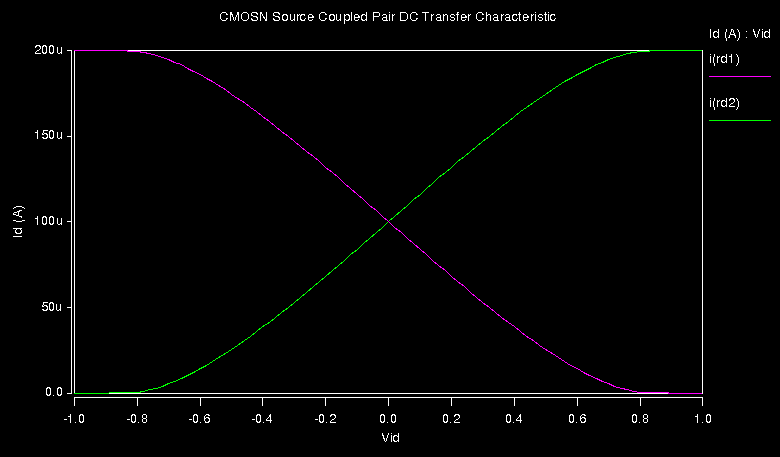
\includegraphics[scale=0.5]{./comsrc.png}
\end{center}
\end{figure}

\end{document}
